
  \section{Zielsetzung}
  Ziel dieses Versuchs ist die Bestimmung der Suszeptibilität unterschiedicher
  paramagnetischer Substanzen.

  \section{Theorie}
Die Suszetibilität $\chi$ ist ein Maß für die magnetisierun und
kann aus dem Bahndrehimpuls und
dem Spin der Elektronenhülle berechnet werden.
Sie hängt von der magnetischen Feldstärke und der Temperatur ab.
Hier wird zwischen zwei Arten von Magnetismus unterschieden.
Der Diamagnetismus, der bei allen Atomen auftritt und auf der Induktion
magnetischer Mometnen durch ein von außen angeegtes Magnetfeld beruht
und der Paramagnetismus, der nur bei Atomen, Ionen und Moleküen Auftritt,
deren Drehimpuls nich verschwindet.
Der Gesamtdrehimpuls $\vec{J}$ für ein hinreichend kleines Magnetfeld
setzt sich aus dem Eigendrehimpuls $\vec{S}$ und dem Bahndrehimpuls
$ \vec{L} $ zusammen.
Mit dem Kosinussatz lässt sich das mittlere magnetische Moment bestimmen.
Für hohr Temperaturen ergibt sich die paramagnetische Suszeptibilitätable
\begin{equation}
  \chi = \frac{1}{3k_BT}\cdot\mu_0\mu_B^2g_J^2NJ(J+1)
\end{equation}
Dabei ist N die Zahl der magnetischen Momente und $\symup{g_J}$ für denLandefaktor und
$\mu_B$ für das Bohrsche Magneton.
\begin{equation}
  g_J = \frac{3J(J+1)+(S(S+1)-L(L+1))}{2J(J+1)}
  \label{eqn:gj}
\end{equation}
\begin{equation}
  \mu_B =\frac{e_0}{2m_0}\hslash
\end{equation}
Für den Versuch wird eine Brückenschaltung benötigt.
Sie ist in Abbildung \ref{fig:brue} zu sehen.
\begin{figure}
  \centering
  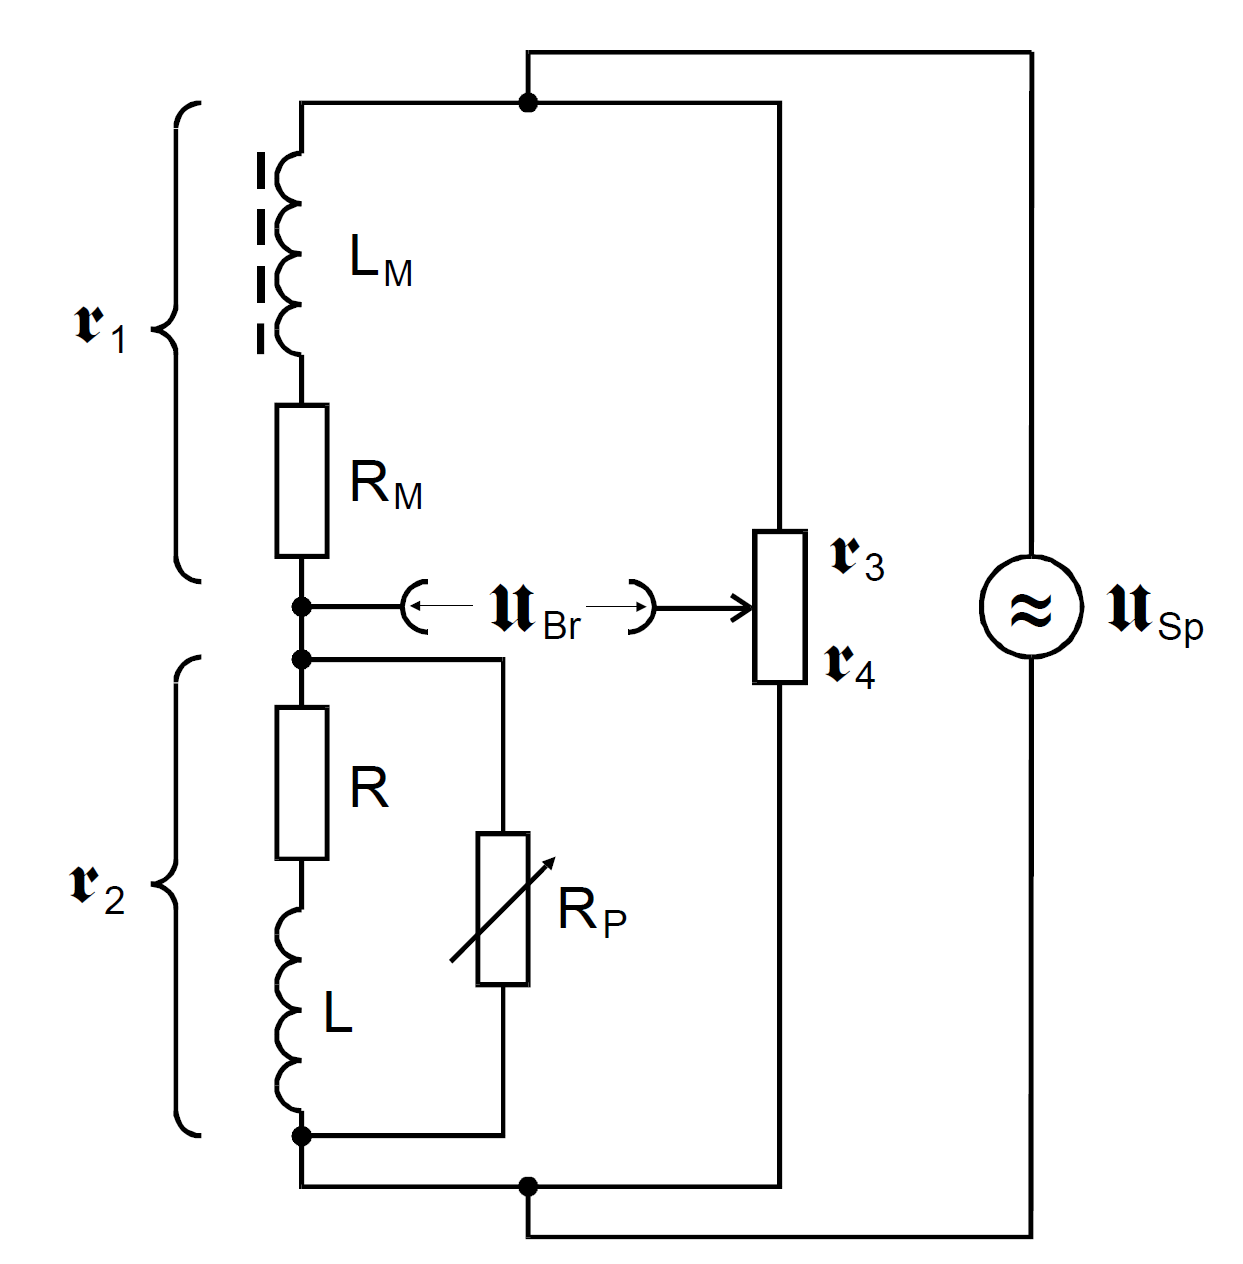
\includegraphics[scale=0.4]{2.png}
  \caption{Die Brrückenschaltung}\cite{Anleitung}
  \label{fig:brue}
\end{figure}
$\symfrak{A}_{Sp}$ ist dabei die Sinusspannung und $\symfrak{A}_{Br}$ die Brückenspannung.
\begin{equation}
  \symfrak{A}_{Br}= \frac{R_4R_1-R_3R_2}{(R_1 + R_2)(R_3 +R_4)}\symfrak{A}_{Sp}
\label{eqn:uu}
\end{equation}
\\
Wird ein Stoff in ddie Spule geschoben ergibt sich die Induktivität zu
\begin{equation}
  L_M = \mu_0 \frac{n^2F}{l}+\chi\mu_0 \frac{n^2Q}{l} = L+ \Delta L
  \label{eqn:L}
\end{equation}
Dabei ist Q der Querschnitt des Stoffes
\begin{equation}
  Q_{real}=Q\frac{p_p}{p_w} ,
  \label{eqn:Q}
\end{equation}
 n die Windungszahl, F der Querschnitt der Spule und
l die Länge der Spule.
\Delta L ist die Änderung der Induktivität nach einführen des Stoffes.\\
Für die Bestimmung der Suszeptibilität gibt es nun zwei Methoden.
Zum einen wird die Nährung $R_3\approx R_4$ verwendet, sodass sich mit (\ref{eqn:L})
\begin{equation}
  \chi = \frac{U_{Br}4l}{U_{Sp}\omega \mu_0 n^2 Q}\sqrt{R^2 +\omega^2\left(\mu_0F \frac{n^2}{l}\right)^2}
\end{equation}
ergibt.
Für $\omega^2L^2>>R^2$ gilt:
\begin{equation}
  \chi = \frac{4FU_{Br}}{QU_{sp}}
  \label{eqn:xs}
\end{equation}
Wird die Brücke durch Variation von $R_3$ zu $\Delta R$ abgeglichen, ergibt sich mit (\ref{eqn:uu})
\begin{equation}
  \chi =\frac{2\Delta R F}{R_3 Q}
  \label{eqn:xw}
\end{equation}
\\
Die Güte Q des Selektivverstärkers ist der Quotient aus der Durchlassfrequenz $\nu_0$ und
der Differenz der Frequenzen $\nu_+$ und $\nu_-$.
\begin{align}
  Q &= \frac{\nu_0}{\nu_+ - \nu_-}
\end{align}


  \section{Durchführung}
Im ersten Teil wird die Filterkurve des Selektiv-Verstärkers untersucht.
Die zu erwartende Filterkurve ist in Abbildung \ref{fig:fil} zu sehen.
\begin{figure}
  \centering
  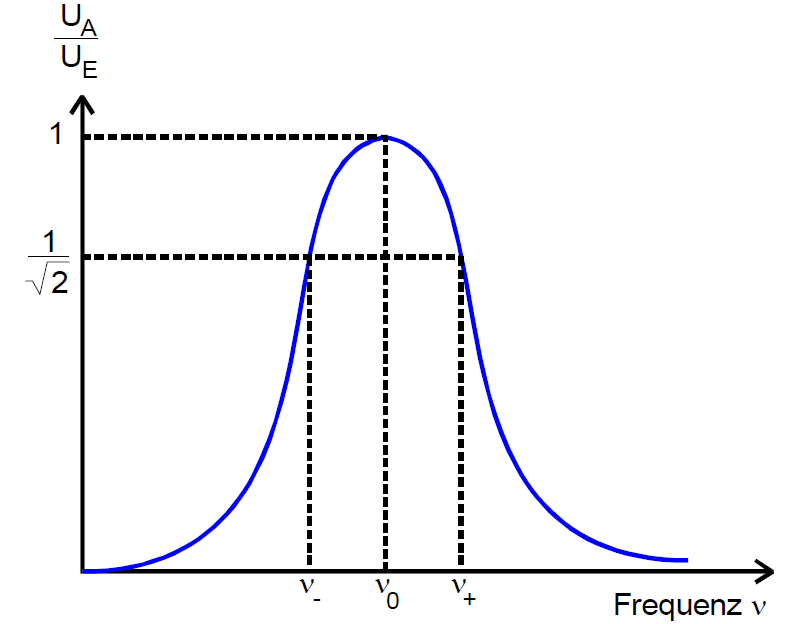
\includegraphics[scale=0.4]{4.png}
  \caption{Filterkurve eines Selektivverstärkers}\cite{Anleitung}
  \label{fig:fil}
\end{figure}
Dafür wird eine Eingangsspannung von $10\,\mathrm{mV}$ angelegt.
Die Durchlassfrequenz wird im Bereich von 30 bis 40 kHz eingestellt und
die zugehörige Ausgangsspannung wird gemessen.

Im nächsten Teil des Versuchs wird die Brückenschaltung zunächst auf Null abgeglichen.
Der Widerstand wird solange verstellt, bis auf dem Oszillographen ein Minimum zu erkennen ist.
Alle Werte werden notiert,
danach wird die Probe C6O12Pr2 in die Spule gebracht.
Der Widerstand wird wieder auf einen Wert gedreht,
sodass ein Minimum zu erkennen ist.
Diese Durchführung wird dreimal wiederholt.
